    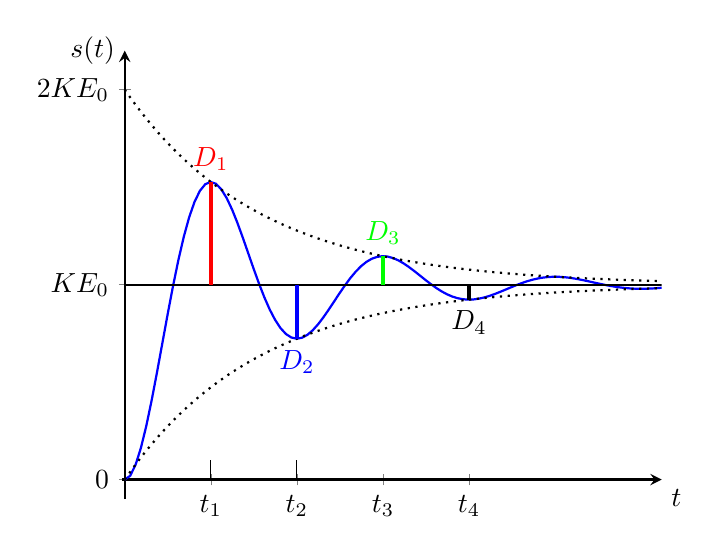
\begin{tikzpicture}                                                                                          
        \pgfmathsetmacro{\a}{0.2}             % amortissement xi                                                 
        \pgfmathsetmacro{\b}{0.96}            % 1-xi^2                                                           
        \pgfmathsetmacro{\w}{0.979795897113}  % w_d=w_0 sqrt(1-xi^2)                                             
        \pgfmathsetmacro{\p}{1.369438406}     % phi =arctan(xi/1-xi^2)                                           
        \pgfmathsetmacro{\tu}{3.206374575405548}    % t1 =                                                       
        \pgfmathsetmacro{\td}{6.4127491508093204}   % t2 = 2*t1                                                  
        \pgfmathsetmacro{\ttt}{9.619123726213981}    % t3 = 3*t1                                                 
        \pgfmathsetmacro{\tq}{12.82549830161864}    % t4 = 4*t1                                                  
        \pgfmathsetmacro{\du}{1.526620599330303}     % dépassement d1                                            
        \pgfmathsetmacro{\dd}{0.72267074436099255}     % dépassement d2                                          
        \pgfmathsetmacro{\dt}{1.146047298816441}     % dépassement d3                                            
        \pgfmathsetmacro{\dq}{0.92308848396671406}     % dépassement d4                                          
                                                                                                                 
        %>>> 1+np.exp(-0.2*np.pi/np.sqrt((1-0.2*0.2)))+1                                                         
        %>>> 1-np.exp(-2*0.2*np.pi/np.sqrt((1-0.2*0.2)))+1                                                       
        %>>> 1+np.exp(-3*0.2*np.pi/np.sqrt((1-0.2*0.2)))+1                                                       
        %>>> 1-np.exp(-4*0.2*np.pi/np.sqrt((1-0.2*0.2)))+1                                                       
        %1.526620599330303                                                                                       
        %0.72267074436099255                                                                                     
        %1.146047298816441                                                                                       
        %0.92308848396671406                                                                                     
                                                                                                                 
        \begin{axis}[                                                                                            
        %ticks=none,                                                                                             
        axis line style = thick,                                                                                 
        %height=9cm,                                                                                             
        %width=12cm,                                                                                             
        axis x line=center,                                                                                      
        axis y line=center,                                                                                      
        xmin=-0.1,                                                                                               
        xmax=20,                                                                                                 
        ymin=-0.1,                                                                                               
        ymax=2.2,                                                                                                
        xlabel={$t$},                                                                                            
        ylabel={$s(t)$},                                                                                         
        xlabel style={below right},                                                                              
        ylabel style={left},                                                                                     
        xticklabels={$t_1$,$t_2$,$t_3$,$t_4$},                                                                   
        xtick={\tu,\td,\ttt,\tq},                                                                                
        yticklabels={0,$KE_0$,$2KE_0$},                                                                          
        ytick={0.001,1,2}                                                                                        
        ]                                                                                                        
        \addplot [thick,color=blue,domain=0:20, samples=101,unbounded coords=jump]{1-((1./\w)*exp(-\a*x)*sin(deg(x)*\w+deg(\p)))};                                                                                                
        \addplot [thick,dotted,domain=0:20, samples=101,unbounded coords=jump]{1+exp(-\a*x)};                    
        \addplot [thick,dotted,domain=0:20, samples=101,unbounded coords=jump]{1-exp(-\a*x)};                    
        \addplot [thick,domain=0:20, samples=101,unbounded coords=jump]{1};                                      
            \draw [ultra thick, red] (axis cs:\tu,1)  -- (axis cs:\tu,\du) node[above] {$D_1$};                  
            \draw [ultra thick, blue] (axis cs:\td,1)  -- (axis cs:\td,\dd) node[below] {$D_2$};                 
            \draw [ultra thick, green] (axis cs:\ttt,1) -- (axis cs:\ttt,\dt) node[above] {$D_3$};               
            \draw [ultra thick, black] (axis cs:\tq,1)  -- (axis cs:\tq,\dq) node[below] {$D_4$};
            \draw (axis cs:\tu,0) -- (axis cs:\tu,0.1);
            \draw (axis cs:\td,0) -- (axis cs:\td,0.1);
        \end{axis}
    \end{tikzpicture}
